\documentclass[12pt, letterpaper]{article}
\usepackage[utf8]{inputenc}
\usepackage[spanish]{babel}
\usepackage{amsmath, amssymb, amsthm, bm}
\usepackage{graphicx}
\usepackage{array}
\usepackage{enumitem}
\usepackage{float}
\usepackage{listings}
\usepackage{xcolor}
\usepackage{tabularx}
\usepackage{booktabs}
%% Sets page size and margins
\usepackage[top=2.5cm,bottom=2.5cm,left=2cm,right=2cm]{geometry}
\usepackage{setspace}
\onehalfspacing
\usepackage{gensymb}
\usepackage{fancyhdr}
\pagestyle{fancy}
\fancyhead[L]{Compiladores}
\fancyhead[C]{Práctica 3}
\fancyhead[R]{Facultad de Ciencias UNAM}
\fancyfoot[C]{\thepage}
\renewcommand{\headrulewidth}{0.4pt}
\renewcommand{\footrulewidth}{0.4pt}

\lstdefinestyle{bashstyle}{
    backgroundcolor=\color{gray!10},
    basicstyle=\small\ttfamily,
    breaklines=true,
    frame=single,
    frameround=tttt
}

\lstset{
    inputencoding=utf8,
    extendedchars=true,
    literate=
        {á}{{\'a}}1
        {é}{{\'e}}1
        {í}{{\'i}}1
        {ó}{{\'o}}1
        {ú}{{\'u}}1
        {Á}{{\'A}}1
        {É}{{\'E}}1
        {Í}{{\'I}}1
        {Ó}{{\'O}}1
        {Ú}{{\'U}}1
        {ñ}{{\~n}}1
        {Ñ}{{\~N}}1
        {ü}{{\"u}}1
        {Ü}{{\"U}}1
}


\title{
    \vspace*{-2.5cm}
    \setlength{\parindent}{0cm} %Indentation 0
    \rule{\linewidth}{0.1mm}
    \vspace*{-1.4cm}
    \begin{center}
        \begin{minipage}{2.5cm}
            \begin{center}
            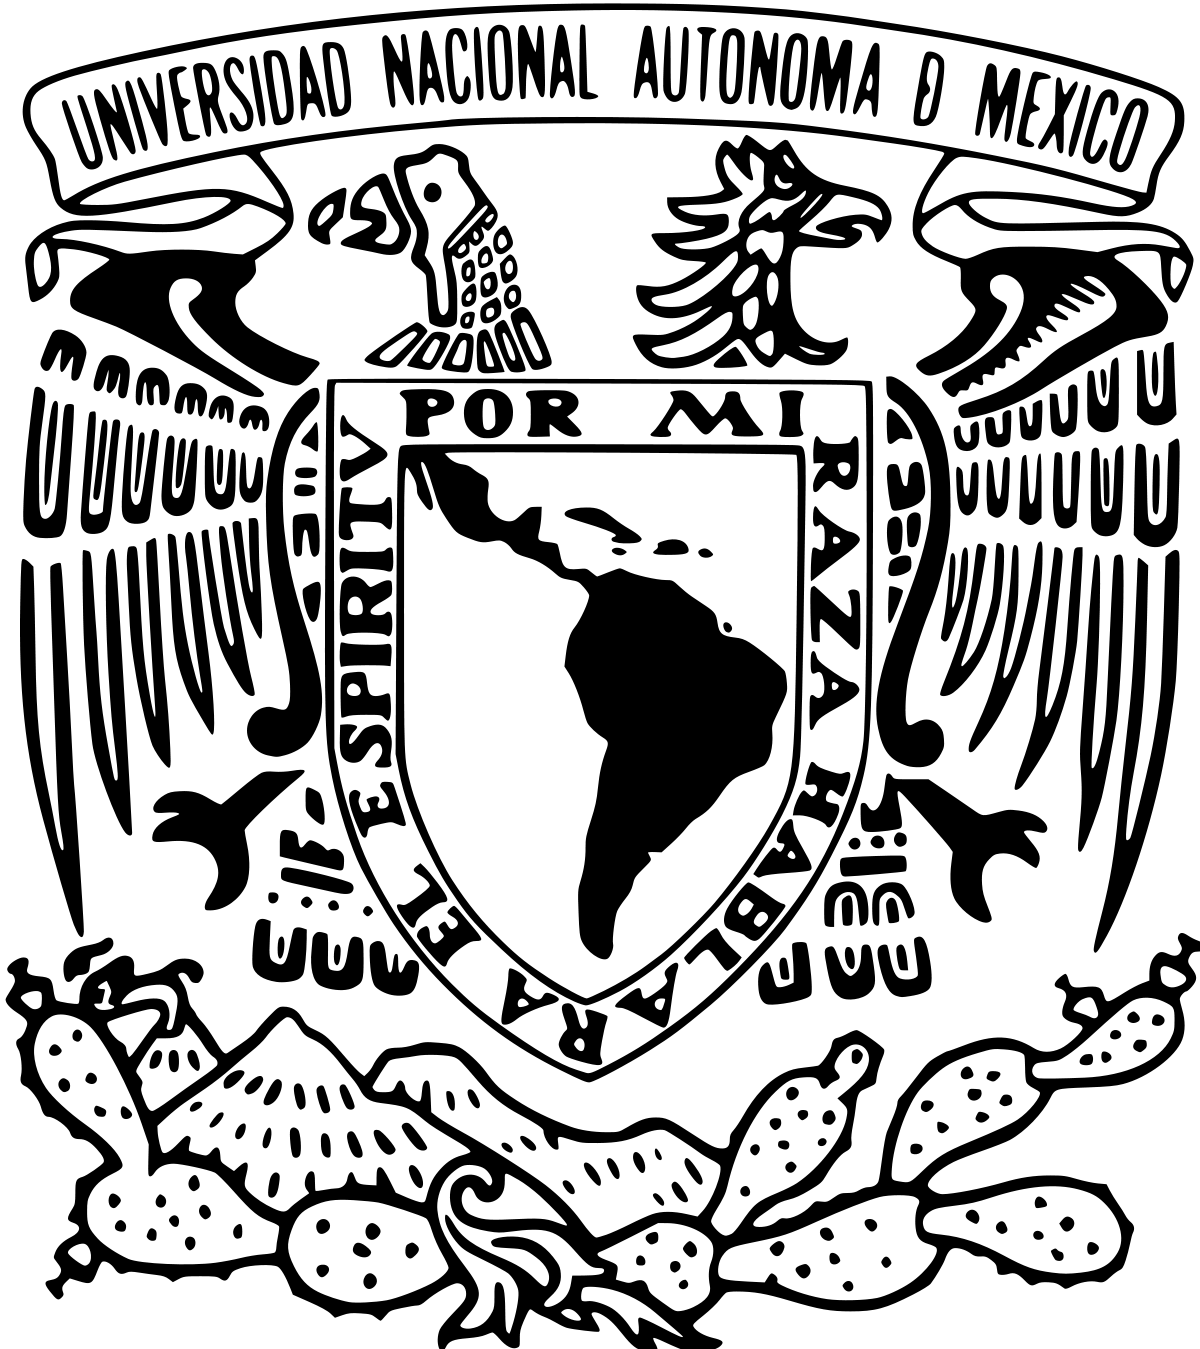
\includegraphics[height=3.4cm]{images/Logo_UNAM.png}
            \end{center}
        \end{minipage}\hfill
        %--------------
        \hspace{0.3cm}
        \begin{minipage}{11cm}
            \begin{center}
            \normalfont \small \textsc{UNIVERSIDAD NACIONAL AUTÓNOMA DE MÉXICO \\ FACULTAD DE CIENCIAS \\ Compiladores } \\
    		\normalsize \textbf{Práctica 3}\\
            \normalsize \textsc{Minimización de un DFA}\\
            \end{center}
        \end{minipage}\hfill
        %--------------
        \begin{minipage}{3cm}
            \begin{center}
            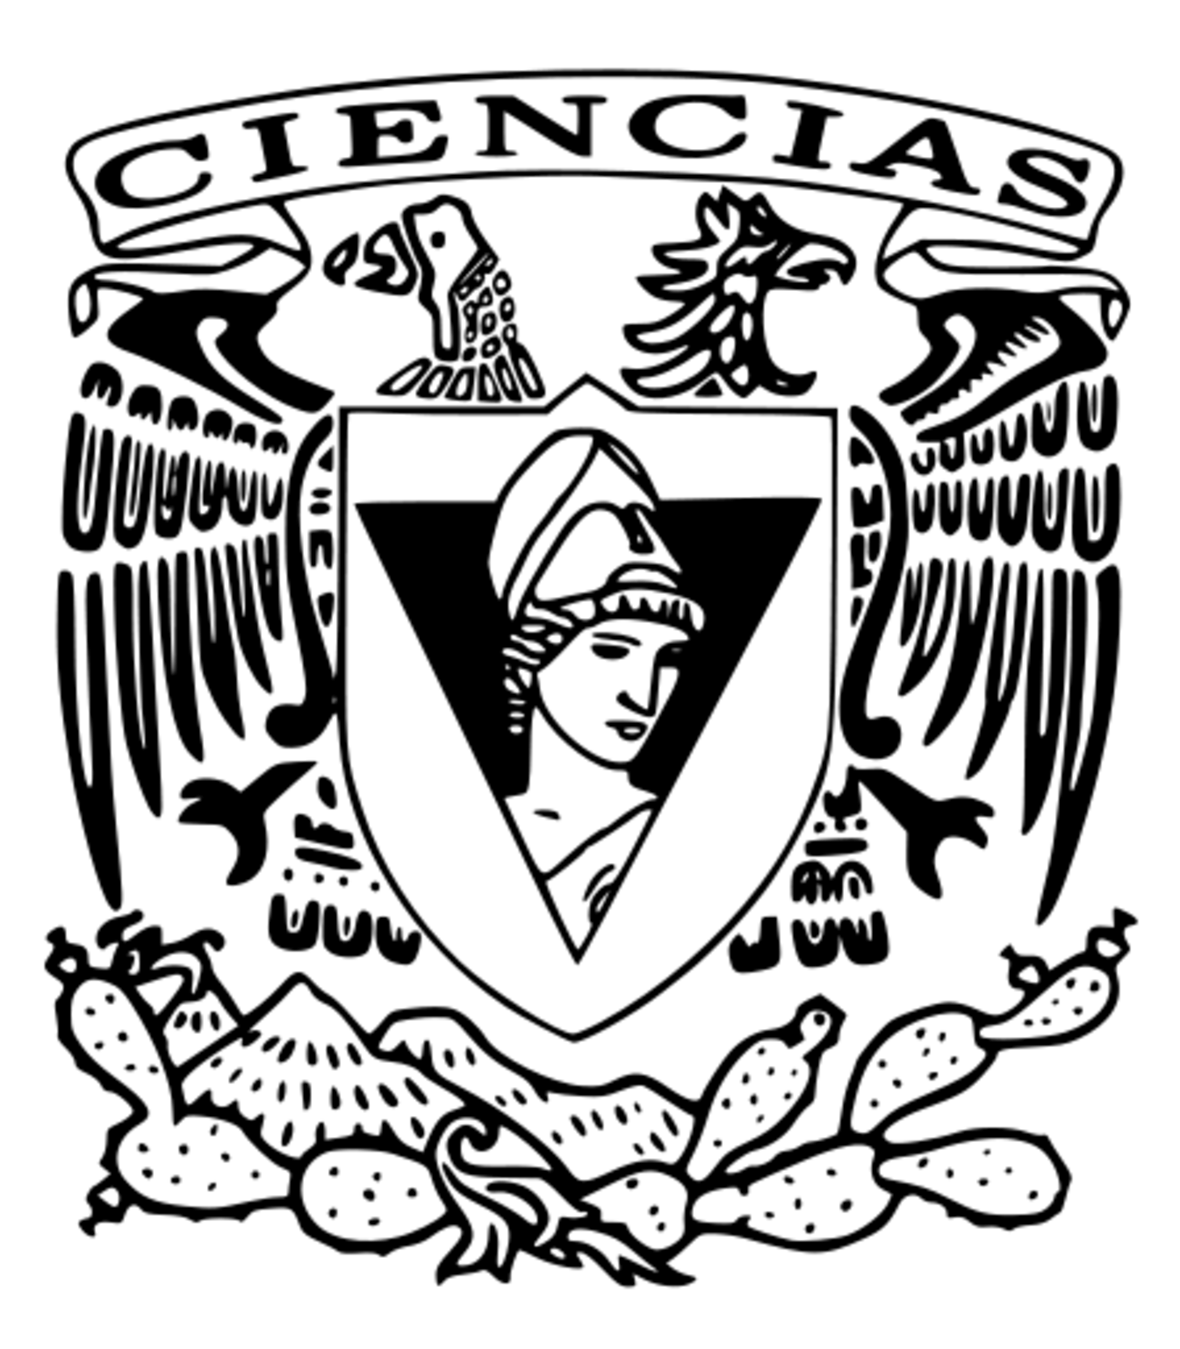
\includegraphics[height=3.6cm]{images/Logo_FC.png}
            \end{center}
        \end{minipage}
    \end{center}
    \vspace*{-0.25cm}
    \rule{\linewidth}{0.1mm}
    \vspace*{0.5cm}
    {\normalsize \textbf{Integrantes:} \par}
    \vspace{-0.5cm}
    \begin{tabular}{{l@{\hspace{1cm}}r}}
        \vspace*{-0.5cm}
        \small Escobar Gonzalez Isaac Giovani & \small 321336400 \\
        \vspace*{-0.5cm}
        \small Garduño Escobar Kevin Jonathan & \small 321070629 \\
        \vspace*{-0.5cm}
        \small Reyes Colín Luis Manuel & \small 321090474 \\
        \vspace*{-0.5cm}
        \small Zaldivar Alanis Rodrigo & \small 424029605
    \end{tabular}
    \date{}
}

\begin{document}
\maketitle
\vspace*{-2.5cm}
\subsection*{Descripción de arquitectura y estructuras de datos}
\noindent El proyecto se organiza en módulos que comparten las estructuras definidas en \texttt{dfa.h}. Un conjunto de estados se representa con la estructura \texttt{state}, un \emph{bitset} respaldado por un arreglo de palabras de 64 bits (\texttt{uint64\_t}); cada bit indica la pertenencia de un estado al conjunto. El autómata \texttt{dfa} agrupa un arreglo de \texttt{state} y una tabla de transiciones \texttt{table[estado][símbolo]} indexada por caracteres, donde el valor $-1$ marca la ausencia de transición. Por convención, el estado inicial siempre ocupa la posición cero del arreglo.

\noindent Tanto la partición $P$ como la cola de trabajo $W$ del algoritmo de Hopcroft se modelan con la estructura \texttt{state\_list}, un arreglo de conjuntos \texttt{state}. Se eligió esta representación (un arreglo de \emph{bitsets}) frente a alternativas como una lista enlazada de conjuntos o un vector de vectores de enteros por tres razones. Primero, por legibilidad: cada bloque de la partición es un único \texttt{state}, la misma abstracción que ya usaba el resto del proyecto. Segundo, por la búsqueda de la preimagen $X = \{q \mid \delta(q,c) \in A\}$, que se resuelve recorriendo los estados y consultando la pertenencia a $A$ en tiempo constante sobre el \emph{bitset}. Tercero, por la manipulación de bloques equivalentes: las operaciones $Y_1 = Y \cap X$ y $Y_2 = Y \setminus X$ se implementan directamente como intersección y diferencia de conjuntos, y la comparación de bloques se reduce a comparar sus palabras.

\noindent La reconstrucción del DFA mínimo se integra de forma natural con la tabla ya existente: a cada clase de equivalencia de la partición final se le asigna un identificador nuevo (la clase que contiene al estado inicial recibe el identificador cero), y la nueva tabla $\delta'$ se llena tomando un representante de cada clase y mapeando el destino de sus transiciones a la clase correspondiente. El subconjunto de estados fusionados se conserva como la unión de los \emph{bitsets} de los miembros, de modo que la tabla impresa sigue mostrando qué estados originales quedaron agrupados.

\subsection*{Instrucciones de compilación y ejecución de pruebas}
\noindent El módulo de minimización se encuentra en \texttt{compilers\_lab/minimization} y se compila con CMake. Desde ese directorio:
\begin{lstlisting}[style=bashstyle]
mkdir -p build && cd build
cmake .. && make
\end{lstlisting}
Esto genera tres ejecutables: \texttt{minimization} (demostración del flujo completo, que imprime la tabla del DFA antes y después de minimizar), \texttt{reachability\_test} (pruebas de eliminación de estados inalcanzables) y \texttt{minimize\_test} (pruebas de la reconstrucción del DFA mínimo). Para ejecutarlos:
\begin{lstlisting}[style=bashstyle]
./reachability_test
./minimize_test
./minimization
\end{lstlisting}
Alternativamente, el \texttt{Dockerfile} incluido compila el proyecto y ejecuta ambas suites de pruebas y la demostración dentro de un contenedor:
\begin{lstlisting}[style=bashstyle]
docker build -t minimization . && docker run --rm minimization
\end{lstlisting}
Seleccionamos 3 expresiones regulares de la lista proporcionada para las pruebas. Mediante la función \texttt{run\_test\_suite} en el archivo \texttt{minimize\_test.c}, se evalua el autómata minimizado contra 20 cadenas por expresión (10 de aceptación y 10 de rechazo).\\
En todas las pruebas se verifica en el código con \texttt{assert} que el número de estados del DFA original fuera mayor o igual que el número de estados del DFA minimizado, es decir, $|Q| \geq |Q^{\prime}|$.\\
De este modo la salida de la ejecución de esta práctica es la siguiente:\\
\begin{lstlisting}[style=bashstyle]
-> docker build -t minimization . && docker run --rm minimization
[+] Building 1.9s (9/9) FINISHED                                                                           docker:default
 => [internal] load build definition from Dockerfile                                                                 0.0s
 => => transferring dockerfile: 540B                                                                                 0.0s
 => [internal] load metadata for docker.io/library/alpine:latest                                                     1.8s
 => [internal] load .dockerignore                                                                                    0.0s
 => => transferring context: 2B                                                                                      0.0s
 => [1/4] FROM docker.io/library/alpine:latest@sha256:294b683cb724975bec92580e1e685676bd4b50bda910ddb8c51d4cabeaec7  0.0s
 => [internal] load build context                                                                                    0.0s
 => => transferring context: 462B                                                                                    0.0s
 => CACHED [2/4] RUN apk add --no-cache gcc musl-dev make cmake                                                      0.0s
 => CACHED [3/4] WORKDIR /app                                                                                        0.0s
 => CACHED [4/4] COPY . .                                                                                            0.0s
 => exporting to image                                                                                               0.0s
 => => exporting layers                                                                                              0.0s
 => => writing image sha256:7f73fac2a22c3700c3cfb07cdbb12c6a66a79173bec6f32fa877ab8e6b31abae                         0.0s
 => => naming to docker.io/library/minimization                                                                      0.0s
-- The C compiler identification is GNU 15.2.0
-- Detecting C compiler ABI info
-- Detecting C compiler ABI info - done
-- Check for working C compiler: /usr/bin/cc - skipped
-- Detecting C compile features
-- Detecting C compile features - done
-- Configuring done (0.3s)
-- Generating done (0.0s)
-- Build files have been written to: /app/build
[  6%] Building C object CMakeFiles/minimization.dir/src/main.c.o
[ 12%] Building C object CMakeFiles/minimization.dir/src/dfa.c.o
[ 18%] Building C object CMakeFiles/minimization.dir/src/reachability.c.o
[ 25%] Building C object CMakeFiles/minimization.dir/src/hopcroft.c.o
[ 31%] Building C object CMakeFiles/minimization.dir/src/minimize.c.o
[ 37%] Linking C executable minimization
[ 37%] Built target minimization
[ 43%] Building C object CMakeFiles/reachability_test.dir/src/reachability_test.c.o
[ 50%] Building C object CMakeFiles/reachability_test.dir/src/dfa.c.o
[ 56%] Building C object CMakeFiles/reachability_test.dir/src/reachability.c.o
[ 62%] Linking C executable reachability_test
[ 62%] Built target reachability_test
[ 68%] Building C object CMakeFiles/minimize_test.dir/src/minimize_test.c.o
[ 75%] Building C object CMakeFiles/minimize_test.dir/src/dfa.c.o
[ 81%] Building C object CMakeFiles/minimize_test.dir/src/reachability.c.o
[ 87%] Building C object CMakeFiles/minimize_test.dir/src/hopcroft.c.o
[ 93%] Building C object CMakeFiles/minimize_test.dir/src/minimize.c.o
[100%] Linking C executable minimize_test
[100%] Built target minimize_test
INICIANDO SUITE DE PRUEBAS DE ALCANZABILIDAD (ROL A)

=== Executing test 1: Unreachable state ===
--- Estados inalcanzables detectados: ---
Estado descartado: 2
El estado 2 no es alcanzable desde el estado inicial 0.
-> Test 1 PASO exitosamente (Estados reducidos de 3 a 2).

=== Ejecutando Test 2: Autobucle y arista hacia q0 ===
--- Estados inalcanzables detectados: ---
El DFA no contiene estados inalcanzables. Se conservan los 3 estados.
-> Test 2 PASO exitosamente (Estados reducidos de 3 a 3).

TODAS LAS PRUEBAS UNITARIAS PASARON CORRECTAMENTE.
Pruebas de reconstrucción del DFA mínimo

Prueba 1: fusión de estados equivalentes
--- Estados inalcanzables detectados: ---
El DFA no contiene estados inalcanzables. Se conservan los 6 estados.
  ok: 6 estados reducidos a 3.

Prueba 2: estado inalcanzable + minimización
--- Estados inalcanzables detectados: ---
Estado descartado: 6
El estado 6 no es alcanzable desde el estado inicial 0.
  ok: 7 -> 6 alcanzables -> 3 mínimo.

Prueba 3: DFA ya mínimo
--- Estados inalcanzables detectados: ---
El DFA no contiene estados inalcanzables. Se conservan los 2 estados.
  ok: se conservan 2 estados.

Todas las pruebas pasaron correctamente.

Pruebas con expresiones regulares

Prueba de regex: (a|b)*abb - Cadenas que terminan en abb

DFA antes de minimizar:

-- Transiciones --
---------------------------------------
 Estado |  'a'  |  'b'  | Acepta | Subconjunto NFA
---------------------------------------
 ->q0   |  q1   |  q0   |   NO    | { 0 }
   q1   |  q1   |  q2   |   NO    | { 1 }
   q2   |  q1   |  q3   |   NO    | { 2 }
   q3   |  q1   |  q0   |   SI    | { 3 }
   q4   |  q1   |  q0   |   NO    | { 4 }
   q5   |  q1   |  q0   |   NO    | { 5 }
---------------------------------------

--- Estados inalcanzables detectados: ---
Estado descartado: 4
El estado 4 no es alcanzable desde el estado inicial 0.
Estado descartado: 5
El estado 5 no es alcanzable desde el estado inicial 0.

DFA después de minimizar:

-- Transiciones --
---------------------------------------
 Estado |  'a'  |  'b'  | Acepta | Subconjunto NFA
---------------------------------------
 ->q0   |  q3   |  q0   |   NO    | { 0 }
   q1   |  q3   |  q0   |   SI    | { 3 }
   q2   |  q3   |  q1   |   NO    | { 2 }
   q3   |  q3   |  q2   |   NO    | { 1 }
---------------------------------------

Número de estados: |Q| original=6, |Q'| minimizado=4

[Corriendo Casos de Aceptación]
Cadena "abb": PASS
Cadena "aabb": PASS
Cadena "aaabb": PASS
Cadena "babb": PASS
Cadena "abababb": PASS
Cadena "ababb": PASS
Cadena "aababb": PASS
Cadena "bbaabb": PASS
Cadena "bbbbabb": PASS
Cadena "ababababb": PASS

[Corriendo Casos de Rechazo]
Cadena "": PASS
Cadena "a": PASS
Cadena "b": PASS
Cadena "ab": PASS
Cadena "aab": PASS
Cadena "ba": PASS
Cadena "aaa": PASS
Cadena "bbb": PASS
Cadena "abab": PASS
Cadena "aabba": PASS

Resultados: 20/20 pruebas superadas.

Prueba de regex: (0|1)*01(0|1)* - Cadenas que contienen la subcadena 01

DFA antes de minimizar:

-- Transiciones --
---------------------------------------
 Estado |  '0'  |  '1'  | Acepta | Subconjunto NFA
---------------------------------------
 ->q0   |  q1   |  q0   |   NO    | { 0 }
   q1   |  q1   |  q2   |   NO    | { 1 }
   q2   |  q3   |  q4   |   SI    | { 2 }
   q3   |  q3   |  q4   |   SI    | { 3 }
   q4   |  q3   |  q4   |   SI    | { 4 }
---------------------------------------

--- Estados inalcanzables detectados: ---
El DFA no contiene estados inalcanzables. Se conservan los 5 estados.

DFA después de minimizar:

-- Transiciones --
---------------------------------------
 Estado |  '0'  |  '1'  | Acepta | Subconjunto NFA
---------------------------------------
 ->q0   |  q2   |  q0   |   NO    | { 0 }
   q1   |  q1   |  q1   |   SI    | { 2, 3, 4 }
   q2   |  q2   |  q1   |   NO    | { 1 }
---------------------------------------

Número de estados: |Q| original=5, |Q'| minimizado=3

[Corriendo Casos de Aceptación]
Cadena "01": PASS
Cadena "001": PASS
Cadena "101": PASS
Cadena "010": PASS
Cadena "1010": PASS
Cadena "0101": PASS
Cadena "10101": PASS
Cadena "01010": PASS
Cadena "101010": PASS
Cadena "01010": PASS

[Corriendo Casos de Rechazo]
Cadena "": PASS
Cadena "0": PASS
Cadena "1": PASS
Cadena "00": PASS
Cadena "11": PASS
Cadena "000": PASS
Cadena "111": PASS
Cadena "1100": PASS
Cadena "55555555": PASS
Cadena "11111111": PASS

Resultados: 20/20 pruebas superadas.

Prueba de regex: (0|10*1)* - Cadenas que tienen un número par de 1s

DFA antes de minimizar:

-- Transiciones --
---------------------------------------
 Estado |  '0'  |  '1'  | Acepta | Subconjunto NFA
---------------------------------------
 ->q0   |  q1   |  q2   |   SI    | { 0 }
   q1   |  q0   |  q3   |   SI    | { 1 }
   q2   |  q2   |  q0   |   NO    | { 2 }
   q3   |  q3   |  q1   |   NO    | { 3 }
---------------------------------------

--- Estados inalcanzables detectados: ---
El DFA no contiene estados inalcanzables. Se conservan los 4 estados.

DFA después de minimizar:

-- Transiciones --
---------------------------------------
 Estado |  '0'  |  '1'  | Acepta | Subconjunto NFA
---------------------------------------
 ->q0   |  q0   |  q1   |   SI    | { 0, 1 }
   q1   |  q1   |  q0   |   NO    | { 2, 3 }
---------------------------------------

Número de estados: |Q| original=4, |Q'| minimizado=2

[Corriendo Casos de Aceptación]
Cadena "": PASS
Cadena "00": PASS
Cadena "11": PASS
Cadena "0000": PASS
Cadena "1111": PASS
Cadena "0011": PASS
Cadena "1100": PASS
Cadena "0101": PASS
Cadena "1010": PASS
Cadena "1001": PASS

[Corriendo Casos de Rechazo]
Cadena "10101": PASS
Cadena "1": PASS
Cadena "01": PASS
Cadena "10": PASS
Cadena "001": PASS
Cadena "111110": PASS
Cadena "01011": PASS
Cadena "100": PASS
Cadena "1110": PASS
Cadena "0001": PASS

Resultados: 20/20 pruebas superadas.

Todas las pruebas de expresiones regulares pasaron correctamente.
Minimización de un DFA

DFA antes de minimizar:

-- Transiciones --
---------------------------------------
 Estado |  '0'  |  '1'  | Acepta | Subconjunto NFA
---------------------------------------
 ->q0   |  q1   |  q2   |   NO    | { 0 }
   q1   |  q0   |  q3   |   NO    | { 1 }
   q2   |  q4   |  q5   |   SI    | { 2 }
   q3   |  q4   |  q5   |   SI    | { 3 }
   q4   |  q4   |  q5   |   SI    | { 4 }
   q5   |  q5   |  q5   |   NO    | { 5 }
   q6   |  q6   |  q6   |   NO    | { 6 }
---------------------------------------


Eliminación de estados inalcanzables:
--- Estados inalcanzables detectados: ---
Estado descartado: 6
El estado 6 no es alcanzable desde el estado inicial 0.

Refinamiento de particiones (Hopcroft):
Clases de equivalencia encontradas: 3

DFA después de minimizar:

-- Transiciones --
---------------------------------------
 Estado |  '0'  |  '1'  | Acepta | Subconjunto NFA
---------------------------------------
 ->q0   |  q0   |  q1   |   NO    | { 0, 1 }
   q1   |  q1   |  q2   |   SI    | { 2, 3, 4 }
   q2   |  q2   |  q2   |   NO    | { 5 }
---------------------------------------

Estados: 7 (original) -> 6 (alcanzable) -> 3 (mínimo)
\end{lstlisting}

\subsection*{Bitácora de casos límite y depuración}
\noindent Para asegurarse que el algoritmo de minimización sea efectivo, se realizó la detección de estados inalcanzables mediante una búsqueda por profundidad del autómata dado su estado inicial, el cual se asume que es el estado cero, en la que se marcan los estados alcanzables. Posteriormente al DFS, se reconstruye el autómata con base en los estados que sí son alcanzables. Esto debido a que nuestros DFAs asumen estados indexados consecutivamente desde cero hasta el número total de estados. En caso de haber reutilizado la tabla de transición del autómata original, quedarían estados inalcanzables. 
En caso de que todos los estados sean alcanzables, dado el cómputo realizado además de que se optó por esta decisión para hacer más efectivo el manejo de memoria, de todas maneras se regresa la reconstrucción del autómata.

\noindent Durante el refinamiento de particiones de Hopcroft, tuvimos como principal dificultad la manipulación de la memoria dinámica en los subconjuntos (\textit{bitsets}) y es que actualizar la partición $P$ y la cola $W$ por referencia directa causaba errores de segmentación al liberar bloques compartidos; esto se corrigió aplicando estrictamente \texttt{state\_clone} y \texttt{state\_free} en cada inserción o reemplazo. Adicionalmente, se previno un ciclo innecesario al buscar la preimagen $X = \{q \mid \delta(q,c) \in A\}$, agregando un salto anticipado (\texttt{continue}) para descartar de inmediato los casos donde $X$ resultaba vacía.

\subsection*{Limitaciones conocidas y deuda técnica}
\noindent En la definición de los DFAs, se asume constante el máximo de símbolos en el alfabeto y de estados; el alfabeto máximo está dado por la cantidad de símbolos totales representados por char y los estados por 128. En algunas funciones, como en aquella cuyo propósito es crear un nuevo autómata sin estados inalcanzables, no se hace uso de nuestra función que nos devuelve el alfabeto para reducir los casos de consulta a la función de transición. Por cada estado, se recorre su fila completa, lo cual aumenta el número de operaciones en la gran mayoría de los casos. El rendimiento se ve especialmente afectado en casos en los que el alfabeto del autómata es considerablemente pequeño, como en el caso en el cual este tiene cardinalidad dos. 

\noindent Respecto a la partición lógica del algoritmo, modelar la cola de trabajo $W$ sobre un arreglo estático contiguo (\texttt{state\_list}) facilita la lectura pero puede empeorar el rendimiento. Esto se debe a que la extracción del primer elemento (\texttt{queue\_pop}) obliga a realizar un corrimiento secuencial de todos los elementos restantes, es decir, nos resulta en una complejidad de $O(N)$ por cada operación. Esto podría mejorarse en una refactorización futura implementando un búfer circular o una lista enlazada para la cola de trabajo, lo que permitiría desencolar en tiempo constante.

\newpage
\subsection*{Validación de Trabajo Presencial / Reposición Teórica}

\begin{center}
    {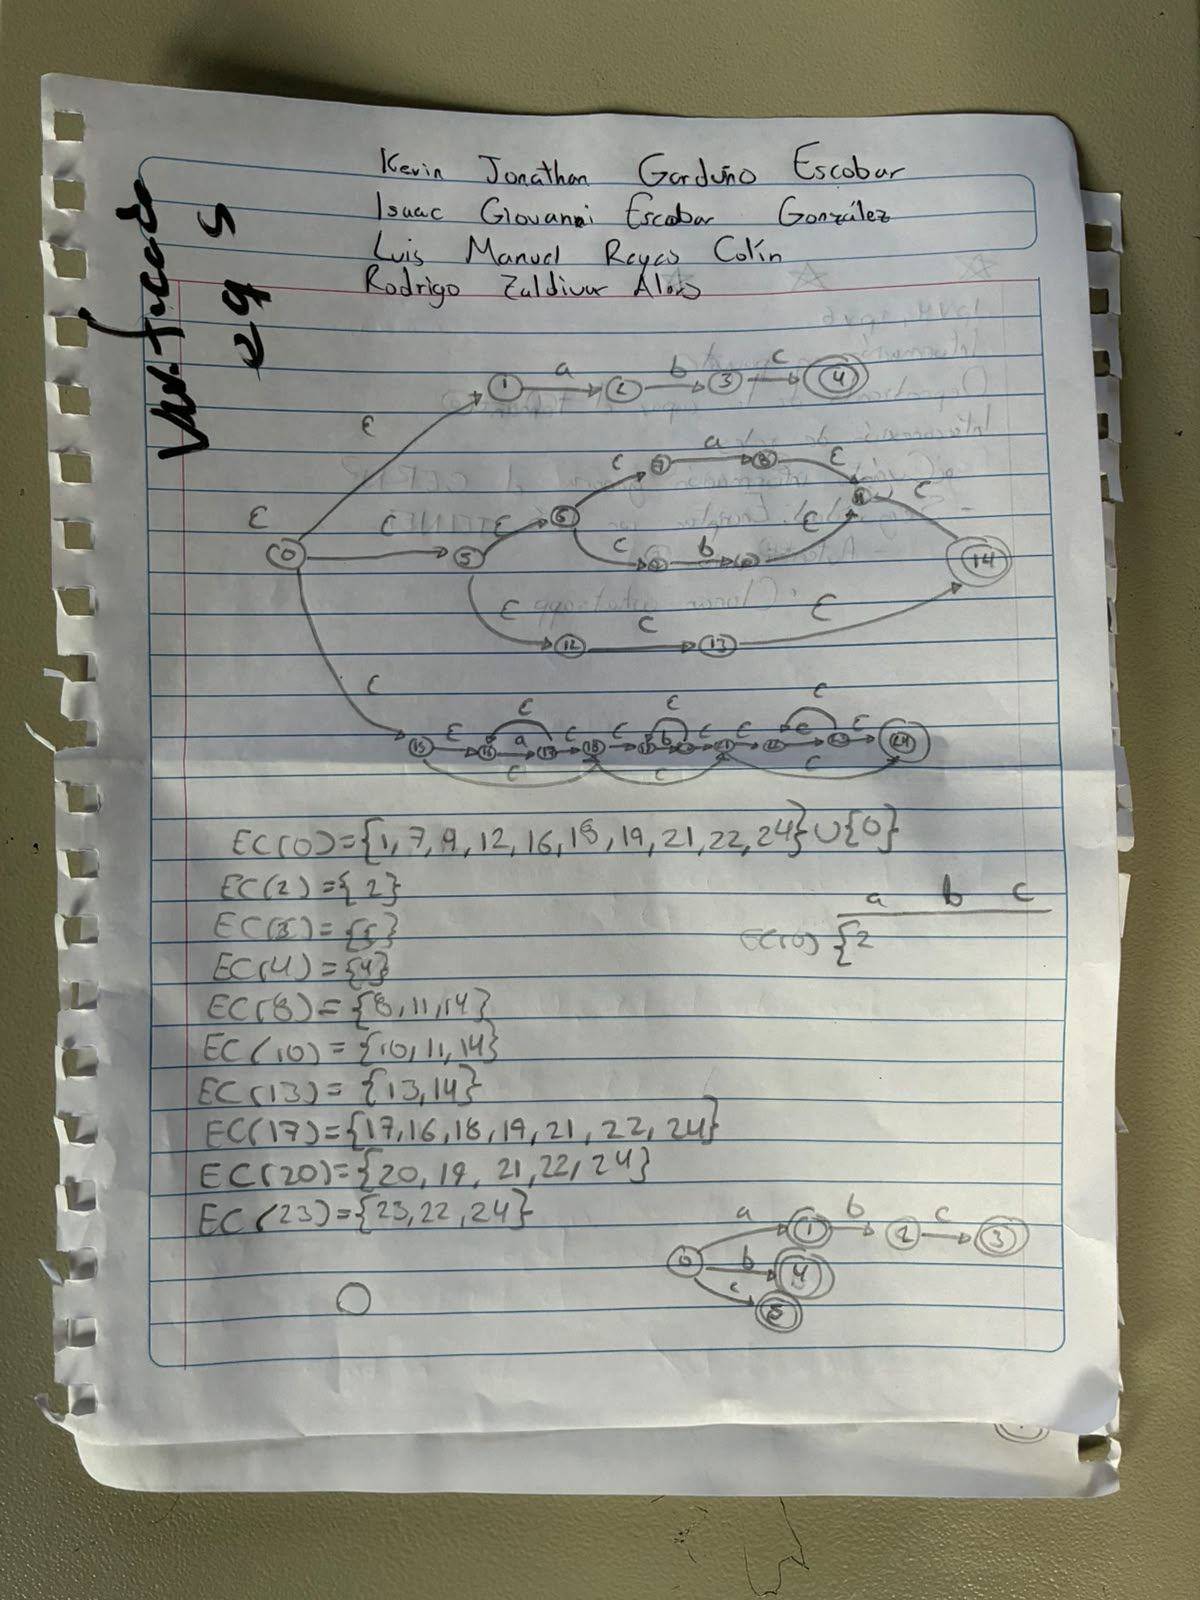
\includegraphics[height=20cm]{images/validacionEquipo.jpg}}
\end{center}

\newpage
\subsection*{Evaluación de la Práctica}
\noindent Grado de acuerdo con cada una de las siguientes afirmaciones utilizando una escala de 1 a 5, donde:
\begin{itemize}
    \item 1: Totalmente en desacuerdo
    \item 2: En desacuerdo
    \item 3: Neutral
    \item 4: De acuerdo
    \item 5: Totalmente de acuerdo
\end{itemize}

\begin{table}[H]
    \centering
    \begin{tabularx}{\textwidth}{|X|c|c|c|c|c|}
        \hline
        \textbf{Criterio / Afirmación} & \textbf{1} & \textbf{2} & \textbf{3} & \textbf{4} & \textbf{5} \\
        \hline
        Los conceptos y habilidades desarrollados en esta práctica son relevantes para mi formación profesional. &  &  & \checkmark &  &  \\
        \hline
        El trabajo realizado me permitió comprender de forma práctica la teoría revisada en clase. &  &  &  & \checkmark &  \\
        \hline
        Las actividades y problemáticas planteadas durante la sesión resultaron atractivas y motivadoras. &  &  & \checkmark &  &  \\
        \hline
        El enfoque práctico y los retos propuestos captaron mi interés a lo largo del desarrollo. &  &  &  & \checkmark &  \\
        \hline
        El nivel de complejidad técnica fue adecuado respecto a los conocimientos y recursos previos disponibles. &  &  &  & \checkmark &  \\
        \hline
        La claridad de la guía permitió realizar la práctica de manera fluida y sin bloques innecesarios. &  &  & \checkmark &  &  \\
        \hline
    \end{tabularx}
\end{table}

\end{document}
